\documentclass{ctexart}
\PassOptionsToPackage{numbers,compress}{natbib}
% Common packages
\usepackage[utf8]{inputenc} % allow utf-8 input
\usepackage[T1]{fontenc}    % use 8-bit T1 fonts
\usepackage{microtype}
\usepackage{times}
\usepackage{graphicx}
\usepackage{amsmath,amssymb,mathbbol}
% \usepackage{algorithmic}
% \usepackage[linesnumbered,ruled,vlined]{algorithm2e}
\usepackage{acronym}
\usepackage{enumitem}
\usepackage[pagebackref=true,breaklinks=true,colorlinks]{hyperref}
\usepackage{balance}
\usepackage{xspace}
\usepackage{setspace}
\usepackage[skip=3pt,font=small]{subcaption}
\usepackage[skip=3pt,font=small]{caption}
\usepackage[dvipsnames]{xcolor}
\usepackage[capitalise]{cleveref}
\usepackage{booktabs,tabularx,colortbl,multirow,array,makecell}
\usepackage{indentfirst} 
% \usepackage{overpic,wrapfig}

\usepackage{fancyhdr}
\hypersetup{pdfencoding=auto,colorlinks=true,allcolors=black}
\renewcommand{\headrulewidth}{0.5pt}
\renewcommand{\footrulewidth}{0pt}
\fancyhf{}
\fancyhead[C]{}
\fancyhead[C]{}
\fancyfoot[C]{\thepage}

% Handy shorthand
\makeatletter
\DeclareRobustCommand\onedot{\futurelet\@let@token\@onedot}
\def\@onedot{\ifx\@let@token.\else.\null\fi\xspace}
\def\eg{\emph{e.g}\onedot} 
\def\Eg{\emph{E.g}\onedot}
\def\ie{\emph{i.e}\onedot} 
\def\Ie{\emph{I.e}\onedot}
\def\cf{\emph{c.f}\onedot} 
\def\Cf{\emph{C.f}\onedot}
\def\etc{\emph{etc}\onedot} 
\def\vs{\emph{vs}\onedot}
\def\wrt{w.r.t\onedot} 
\def\dof{d.o.f\onedot}
\def\etal{\emph{et al}\onedot}
\makeatother

\definecolor{gray}{gray}{0.9}

% Handy math ops
\DeclareMathOperator*{\argmax}{arg\,max}
\DeclareMathOperator*{\argmin}{arg\,min}
\newcommand{\norm}[1]{\left\Vert #1 \right\Vert}

% % Spacing
\frenchspacing
% \medmuskip=2mu   % reduce spacing around binary operators
% \thickmuskip=3mu % reduce spacing around relational operators
% \setlength{\abovedisplayskip}{3pt}
% \setlength{\belowdisplayskip}{3pt}
% \setlength{\abovecaptionskip}{3pt}
% \setlength{\belowcaptionskip}{3pt}
\setlength\floatsep{0.5\baselineskip plus 3pt minus 2pt}
\setlength\textfloatsep{0.5\baselineskip plus 3pt minus 2pt}
\setlength\dbltextfloatsep{0.5\baselineskip plus 3pt minus 2pt}
\setlength\intextsep{0.5\baselineskip plus 3pt minus 2pt}

\makeatletter
\renewcommand{\paragraph}{%
  \@startsection{paragraph}{4}%
  {\z@}{0ex \@plus 0ex \@minus 0ex}{-1em}%
  {\hskip\parindent\normalfont\normalsize\bfseries}%
}
\makeatother

% Graphics path
\graphicspath{{figures/}}

% Clever references
\crefname{algorithm}{Alg.}{Algs.}
\Crefname{algorithm}{Algorithm}{Algorithms}
\crefname{section}{Sec.}{Secs.}
\Crefname{section}{Section}{Sections}
\crefname{table}{Tab.}{Tabs.}
\Crefname{table}{Table}{Tables}
\crefname{figure}{Fig.}{Fig.}
\Crefname{figure}{Figure}{Figure}

% Acronym
\acrodef{pku}[PKU]{Peking University}
\usepackage[final]{template22}
\setlength{\parindent}{2em}

\title{Lab2-MeshSimpification}
\author{王想 2100013146}
\date{}
\begin{document}
\maketitle

\section{算法实现}
算法大致流程如下:

1. 对每个顶点 $v_i$ ,计算邻居位置的加权平均
$v_i^*=\frac{\sum_{j\in N(i)}w_{ij} v_j}{\sum_{j\in N(i)} w_{ij}}$
其中, $w_{ij}=\cot \alpha_{ij} + \cot \beta_{ij}$, 夹角$\alpha_{ij},\beta_{ij}$见下方示意图。

2. 更新顶点:$v_i=(1-\lambda)v_i+\lambda v_i^*$

3. 重复1-2步,直到迭代次数达到上限

\begin{figure}[htbp]
    \centering
    \centering
    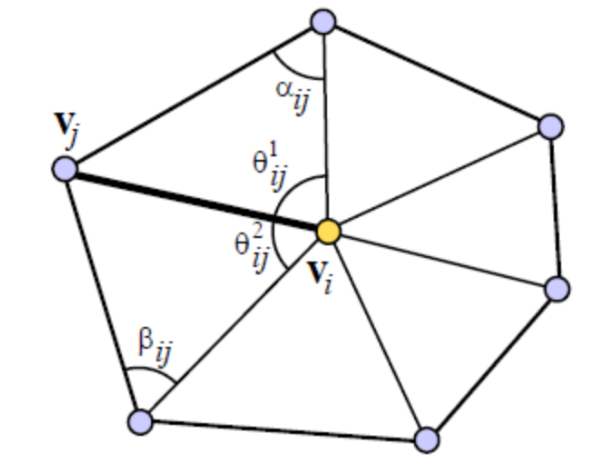
\includegraphics[width=0.6\linewidth]{figures/cotangent.png}
\end{figure}

需要注意的是这里需要在每一次迭代之前先把更新前顶点的位置复制一份保存下来,
在后续更新的计算中,邻居点的位置应该是更新前的邻居顶点的位置。
如果没有留存更新前的顶点坐标就直接改变mesh的顶点坐标,
会导致用新的顶点坐标去更新其他点的坐标,
这些微小的偏差会积累起来导致最后的平滑效果出现较大误差。

\section{Results}
迭代步长$\lambda$越大,平滑程度越大,需要的迭代次数也越小,但相应的缺点是容易过度平滑;
迭代次数$iteration$越大,平滑程度越大,但代价是时间消耗过多,
在我的电脑中串行执行时,迭代一次平均花费21s。
在尝试多组超参之后,我发现小步长、大迭代次数的效果最好。

图2为原网格与平滑后网格的对比,图3为超参$\lambda$的调整对平滑效果的影响对比(这里只展示部分有代表性的超参)。
可以看到,
在参数$\lambda= 0.1,iteration = 10$下,平滑程度不太够,仍显得有点杂乱;
在参数$\lambda= 0.5,iteration = 10$下,兔耳已经被磨平了一部分;
在参数$\lambda= 0.5,iteration = 10$下,兔耳被完全磨平;
在参数$\lambda= 0.1,iteration = 20$下,既保证了平滑效果,又防止了过度平滑。

\begin{figure}[htbp]
    \centering
    \begin{subfigure}[htbp]{0.45\linewidth}
        \centering
        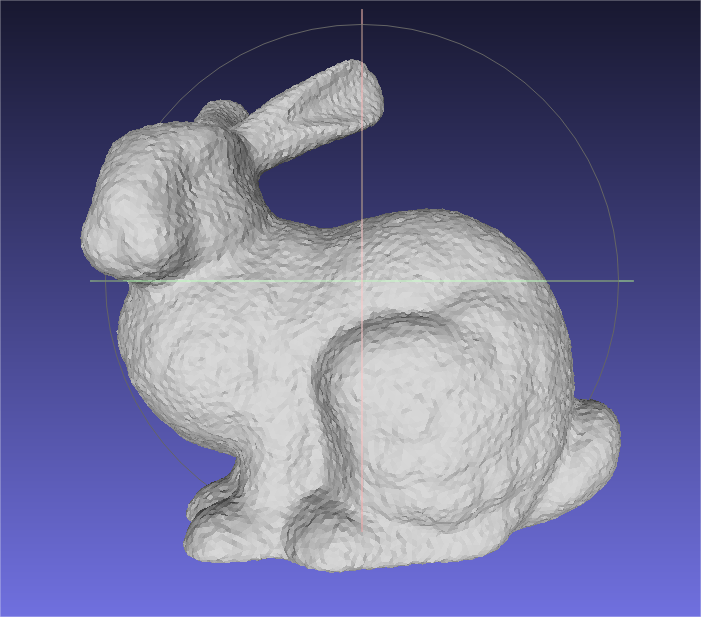
\includegraphics[width=0.9\linewidth]{figures/0.png}
        \caption{\textbf{Origin}}
    \end{subfigure}
    \begin{subfigure}[htbp]{0.45\linewidth}
        \centering
        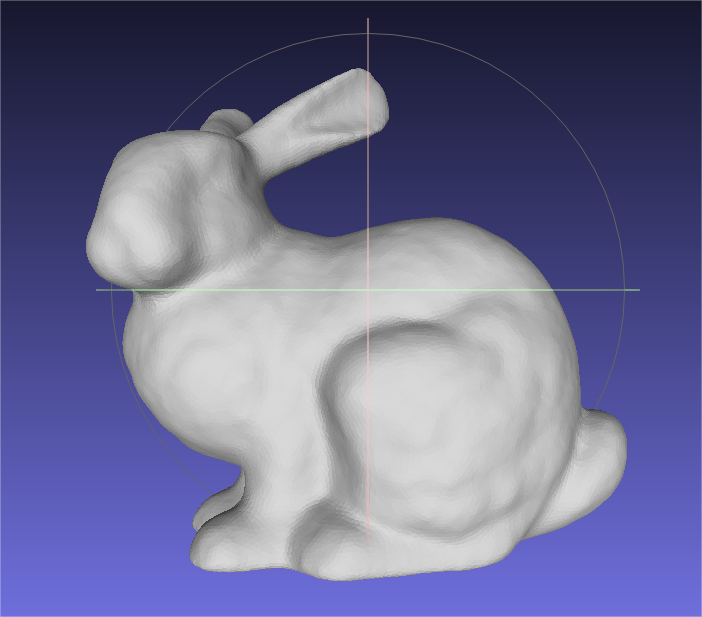
\includegraphics[width=0.9\linewidth]{figures/1-20.png}
        \caption{\textbf{$\lambda$ = 0.1, iteration = 20}}
    \end{subfigure}
    \caption{\textbf{Smooth}}
\end{figure}

\begin{figure}[htbp]
    \centering
    \begin{subfigure}[htbp]{0.24\linewidth}
        \centering
        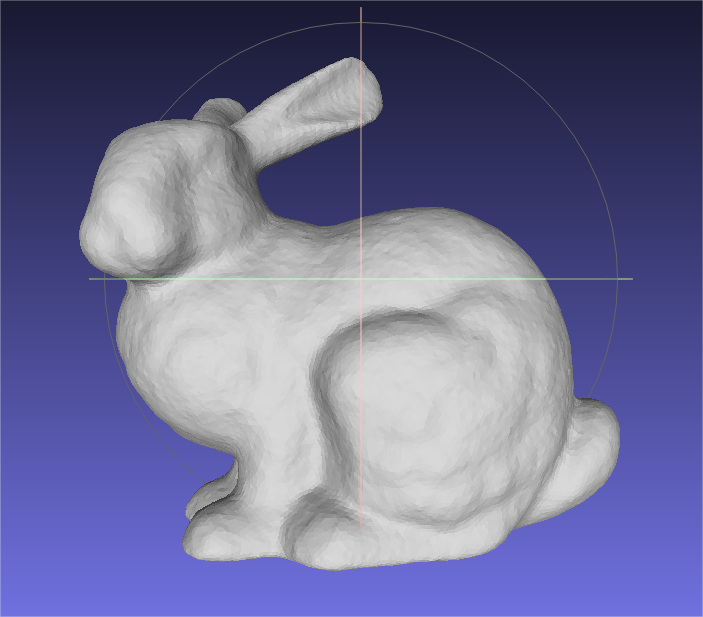
\includegraphics[width=0.9\linewidth]{figures/1.png}
        \caption{\textbf{$\lambda$ = 0.1, iteration = 10}}
    \end{subfigure}
    \begin{subfigure}[htbp]{0.24\linewidth}
        \centering
        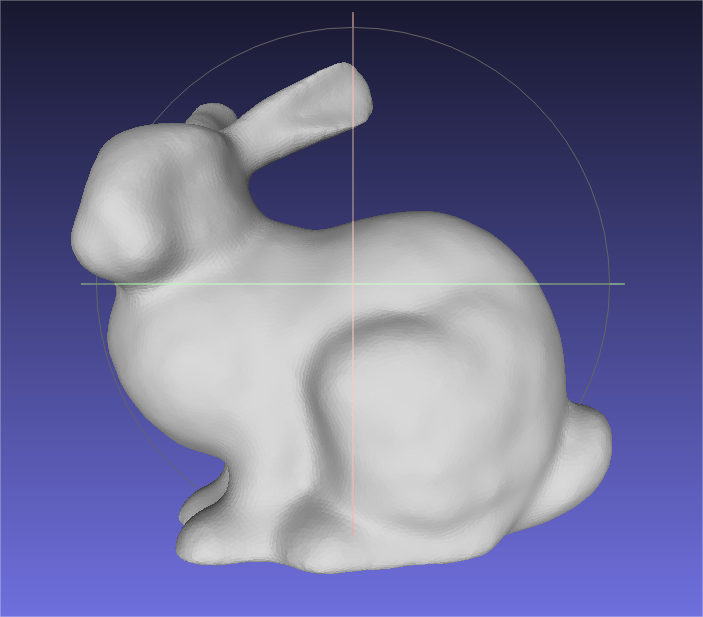
\includegraphics[width=0.9\linewidth]{figures/5.png}
        \caption{\textbf{$\lambda$ = 0.5, iteration = 10}}
    \end{subfigure}
    \begin{subfigure}[htbp]{0.24\linewidth}
        \centering
        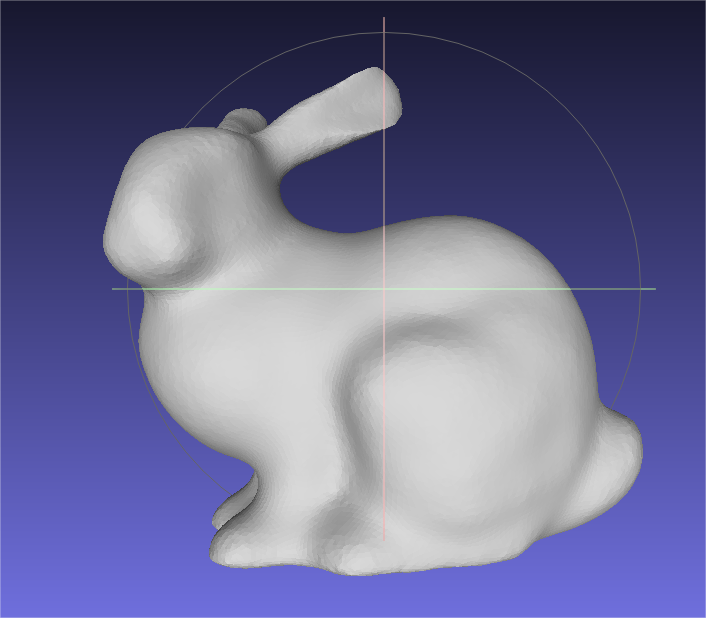
\includegraphics[width=0.9\linewidth]{figures/9.png}
        \caption{\textbf{$\lambda$ = 0.9, iteration = 10}}
    \end{subfigure}
    \begin{subfigure}[htbp]{0.24\linewidth}
        \centering
        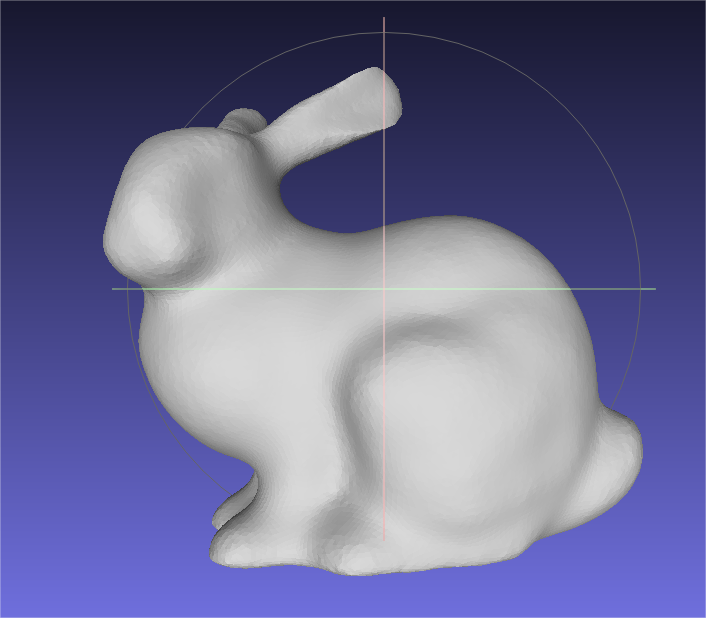
\includegraphics[width=0.9\linewidth]{figures/9.png}
        \caption{\textbf{$\lambda$ = 0.1, iteration = 20}}
    \end{subfigure}
    \begin{subfigure}[htbp]{0.24\linewidth}
        \centering
        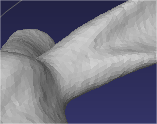
\includegraphics[width=0.9\linewidth]{figures/detail_1.png}
        \caption{\textbf{local detail of fig(a)}}
    \end{subfigure}
    \begin{subfigure}[htbp]{0.24\linewidth}
        \centering
        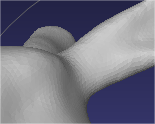
\includegraphics[width=0.9\linewidth]{figures/detail_5.png}
        \caption{\textbf{local detail of fig(b)}}
    \end{subfigure}
    \begin{subfigure}[htbp]{0.24\linewidth}
        \centering
        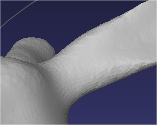
\includegraphics[width=0.9\linewidth]{figures/detail_9.png}
        \caption{\textbf{local detail of fig(c)}}
    \end{subfigure}
    \begin{subfigure}[htbp]{0.24\linewidth}
        \centering
        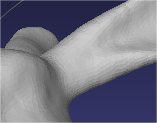
\includegraphics[width=0.9\linewidth]{figures/detail_1-20.png}
        \caption{\textbf{local detail of fig(d)}}
    \end{subfigure}
    \caption{\textbf{Hyperparamerter Tuning}}
\end{figure}

\section{Improvements}
在保存下每一轮迭代更新前顶点的坐标后,
考虑到每一个顶点的更新计算均是平行、独立的,
不会相互影响,于是我们可以采用并行计算分别对每一个点进行更新,
这样会大大加速平滑计算,相较于串行计算能节省大量时间。

\appendix
\section{Appendix}
Requirement: $openmesh,\ numpy$

Running command: $python\ smooth.py$


\end{document}